\chapter{Explainability Results} \label{app:explainability}

\section{Feature Importance} \label{app:feature_importance}

Figure \ref{fig:feature_importance_by_asset} shows the top features grouped by asset according to the feature importance of the surrogate model. 

\begin{figure}
    \centering
    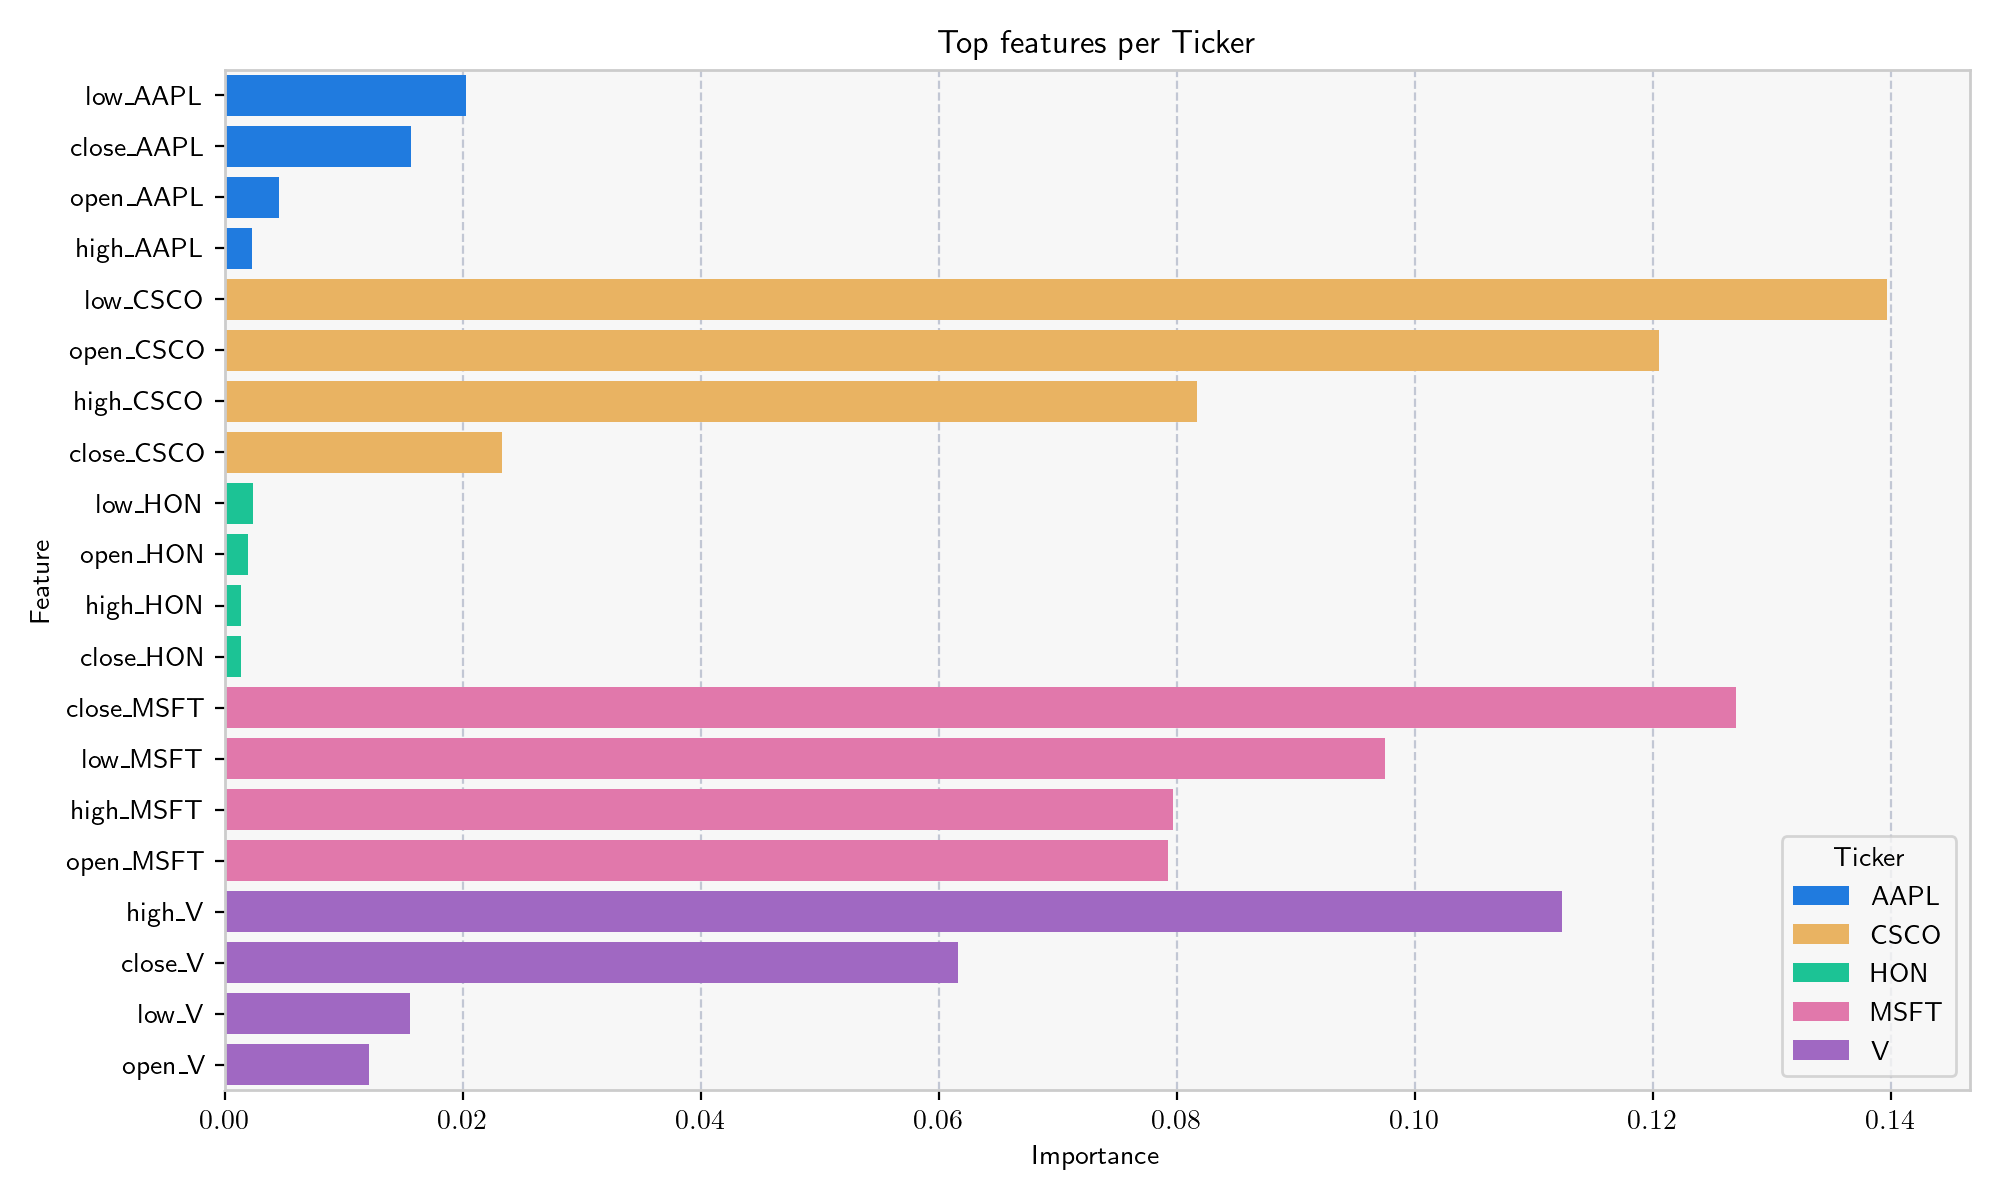
\includegraphics[width=0.8\textwidth]{figures/feature_importance_top_features_by_ticker.png}
    \caption{Top features grouped by asset from the surrogate model according to feature importance.}
    \label{fig:feature_importance_by_asset}
\end{figure}

Figure \ref{fig:mean_feature_importance_by_feature} shows the mean feature importance for each type of feature, i.e. open, close, high and low prices, over the assets.

\begin{figure}
    \centering
    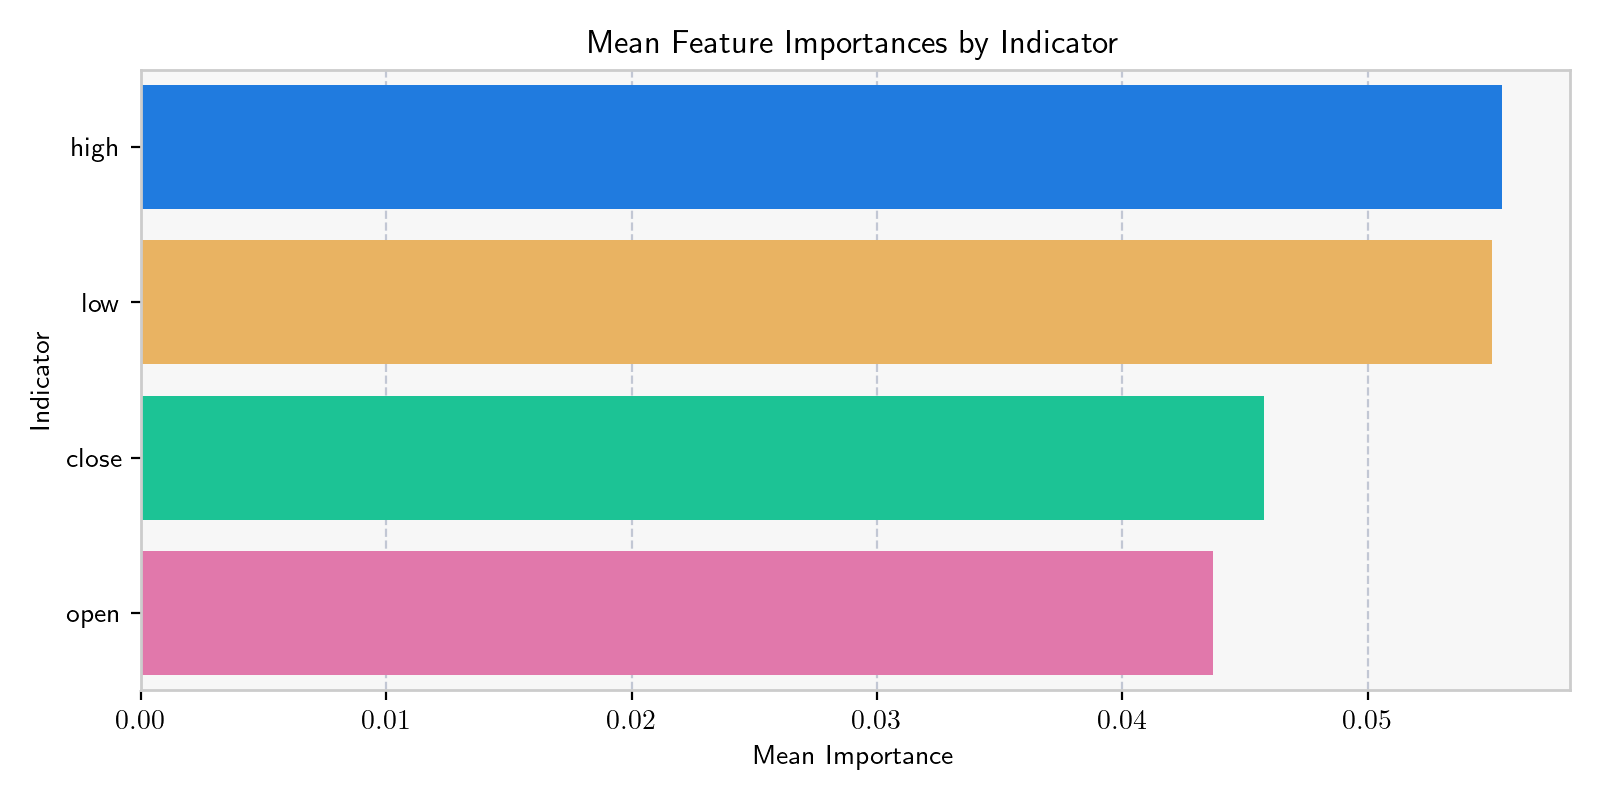
\includegraphics[width=0.8\textwidth]{figures/feature_importance_mean_indicator.png}
    \caption{Mean feature importance per type of feature from the surrogate model.}
    \label{fig:mean_feature_importance_by_feature}
\end{figure}

\clearpage
\section{Local Importance Model-Agnostic Explanation Results} \label{app:lime_explanations}

With the \acrshort{lime} analysis, the explanations for the \acrshort{a2c} algorithm are provided. Since these are local observations, the following figures provide the explanation for the first time step on the test dataset of the assets not included in the main text. Values coloured in orange represent features that contribute positively to the prediction, while blue values indicate features that contribute negatively.

\begin{figure}
    \centering
    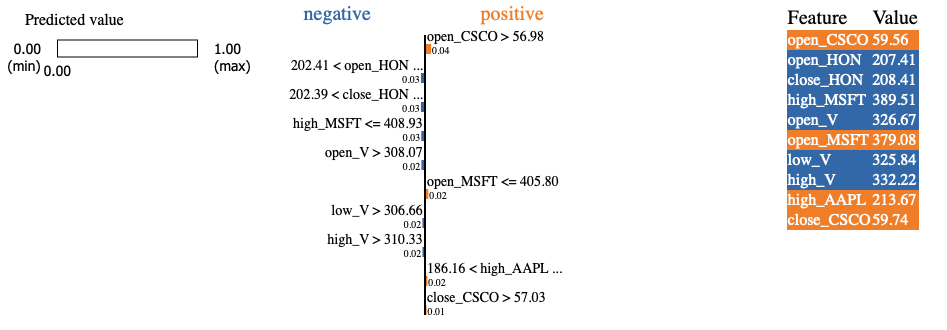
\includegraphics[width=0.8\textwidth]{figures/a2c_lime_aapl.png}
    \label{fig:a2c_lime_aapl}
    \caption{\acrshort{lime} explanations for the \acrshort{a2c} algorithm for a specific observation in the test dataset for the AAPL asset.}
\end{figure}

\begin{figure}
    \centering
    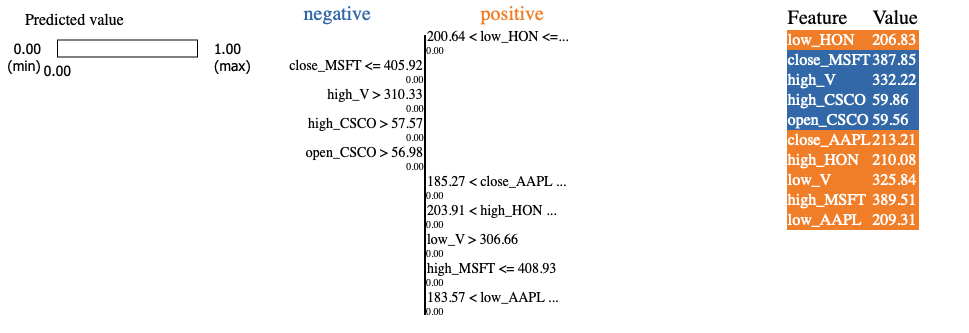
\includegraphics[width=0.8\textwidth]{figures/a2c_lime_csco.png}
    \label{fig:a2c_lime_csco}
    \caption{\acrshort{lime} explanations for the \acrshort{a2c} algorithm for a specific observation in the test dataset for the CSCO asset.}
\end{figure}

\begin{figure}
    \centering
    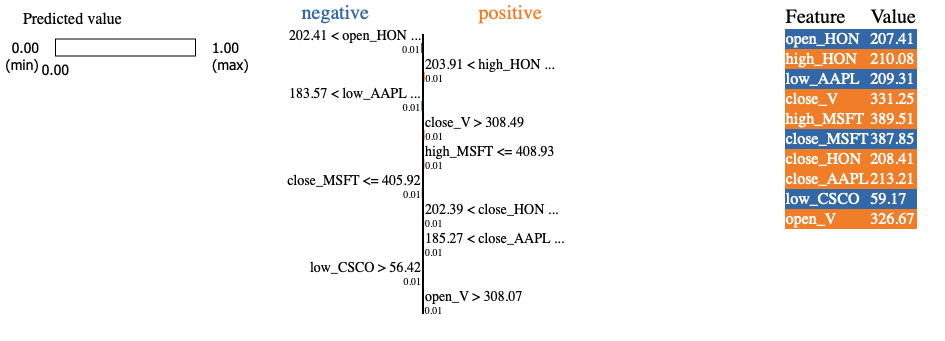
\includegraphics[width=0.8\textwidth]{figures/a2c_lime_hon.png}
    \label{fig:a2c_lime_hon}
    \caption{\acrshort{lime} explanations for the \acrshort{a2c} algorithm for a specific observation in the test dataset for the HON asset.}
\end{figure}

\begin{figure}
    \centering
    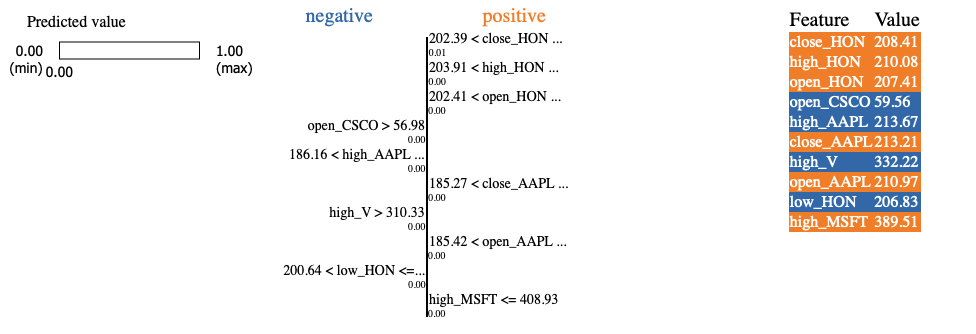
\includegraphics[width=0.8\textwidth]{figures/a2c_lime_v.png}
    \label{fig:a2c_lime_v}
    \caption{\acrshort{lime} explanations for the \acrshort{a2c} algorithm for a specific observation in the test dataset for the V asset.}
\end{figure}

